\documentclass[../main.tex]{subfiles}

\begin{document}

\problem{2}

\givens{}
\(M_\infty = 3.0\)\\
\(T_\infty = 217 \,\unit{\kelvin}\)\\
\(p_\infty = 20 \,\unit{\kilo\pascal}\)\\
\(\gamma=1.4\)\\
\(R = 287\,\unit{\joule/\kilogram\,\kelvin}\)\\
\(c_p = 1000 \, \unit{\joule/\kilogram\,\kelvin}\)\\
\(q_{combustor} = 500 \, \unit{\kilo\joule/\kilogram}\)

\assumptions{}

\begin{enumerate}[label=(\roman*)]
    \item Steady \label{steady}
    \item Inviscid \label{inviscid}
    \item Uniform velocity, pressure, temperature, density, enthalpy, and energy at each \(x\) location. \label{uniform}
    \item The oblique shock from the spike is an attached weak shock from a two-dimensional wedge. \label{oblique}
    \item We will neglect the angularity of the streamline through the inlet. 
        For example, we will assume that the fluid is travelling horizontally between the oblique and normal shocks and between the normal shock and fuel injection. \label{angularity}
    \item Our general isentropic, oblique-shock, and normal-shock equations apply (where appropriate). \label{general}
    \item We will assume that the static Mach number at the inlet of the combustor is the same value throughout the entire combustor.
        \label{constant_mach}
    \item You may use an isentropic relation to calculate the static temperature at the exit of the combustor. \label{combustortemp}
    \item We will utilize one-dimensional flow with heat transfer to obtain the difference in stagnation temperature between the inlet and exit of the combustor from the given constant value of q. \label{combustion}
    \item We will neglect the fuel mixture in the air in the combustor. \label{fuel}
    
\end{enumerate}

\problempart{a} 

Briefly describe how a ramjet works.

\discussion{}
A ramjet is a form of high-speed propulsion system that does not involve any turbomachinery to compress the flow.
Only capable of starting at higher Mach numbers (~3+), a ramjet utilizes a series of oblique and normal shocks (depending on the inlet design) to compress and slow the freestream flow that is being captured for use.
The flow must be slowed to subsonic velocities for ramjet operation, as by definition a ramjet utilizes subsonic combustion.
As in a turbofan or turbojet engine, fuel is injected into the flow, combusted to generate a large pressure and temperature rise, and then accelerated out of a nozzle to convert pressure and thermal energy into kinetic energy that propels a vehicle forward.
Traditional turbomachinery runs into operational issues at high-Mach conditions due to shockwaves generated in the compression section of the flowpath.

\problempart{b} 

A simplified ramjet cycle efficiency is given by:

\[
    \eta = 1 - \left({
    \left({\frac{p_{1,\infty}}{p_{3,\infty}}}\right)^{\frac{\gamma-1}{\gamma}}
    \frac{
        \left({T_{4,\infty} - \left({\frac{p_{3,0}}{p_{1,0}}}\right)^{{\frac{\gamma-1}{\gamma}}}} \cdot T_{3,\infty}\right)
    }{\left({T_{4,\infty}-T_{3,\infty}}\right)}
    }\right)
\]

Use this equation to come up with the optimal spike half angle (to the nearest degree) for the given cruise conditions. 
You must write out your general methodology for the grader.
Include a plot of the efficiency versus spike half angle.

\solution{}

The solution methodology to calculate the ideal inlet spike half angle, \(\theta\), is described below. 
Assumptions \ref{steady}-\ref{uniform} allow us to utilize the simplified 1-D forms of continuity, momentum, and energy, which directly lead to the isentropic, normal shock, and oblique shock relations that will be used in this problem, per assumption \ref{general}.
For brevity, not all calculations are shown.

\textit{Note: All calculations performed in Python, see Appendix \ref{Problem2Python}}.

\begin{enumerate}

    \item For a given freestream Mach number, \(M_\infty\), and a given inlet half angles, \(\theta\), solve for the corresponding shock angle, \(\beta\), per assumption \ref{angularity}. 

    \item Using \(\beta\), determine the component of the incoming Mach normal to the oblique shock, \(M_{1n}\).
    
    \item Use normal shock relationships to calculate the normal component of post-oblique-shock Mach number, \(M_{2n}\), 
    
    \item Use normal shock relationships to calculate the static pressure ratio across the oblique shock, \(\frac{p_2}{p_1}\), as well as the static temperature ratio, \(\frac{T_2}{T_1}\)..
    
    \item With \(M_{2n}\), \(\beta\), and \(\theta\), determine the magnitude of the post-oblique shock Mach number, \(M_2\).
    
    \item Using assumption \ref{angularity}, treat \(M_2\) as normal to the standing normal shock and use normal shock relationships to determine \(M_3\), the Mach number at the entrance to the combustor
    
    \item Use normal shock relationships to calculate \(\frac{p_3}{p_2}\), the post-normal-shock static pressure ratio, as well as the static temperature ratio \(\frac{T_3}{T_2}\).

    \item Solve for \(T_3\) using \(T_3 = \frac{T_3}{T_2} \frac{T_2}{T_1} T_1\) where \(T_1\) is the freestream temperature, \(T_\infty\).

    \item Use isentropic relationships for \(M_3\) and \(T_3\) to calculate the total temperature at the entrance to the combustor, \(T_{t,3}\).
    
    \item Use the energy equation for 1-D flow with heat addition (a.k.a. Rayleigh Flow, assumption \ref{combustion}) to calculate the total temperature at the exit of the combustor, \(T_{t,4}\), recognizing that total enthalpy can be expressed in terms of specific heats and total temperature.

    \[
        h_{t,3} + q = h_{t,4}  
    \]
    \[  
        h = c_p T    
    \]
    \[
        c_p T_{t,3} + q = c_p T_{t,4}     
    \]

    \item Assuming that the Mach number is constant throughout the combustor (per assumption \ref{constant_mach}), use isentropic relationships to solve for \(T_4\) with \(M_4=M_3\) (assumption \ref{combustortemp}), neglecting the increased mass from fuel injection (assumption \ref{fuel}).
    
    \item Calculate the ramjet cycle efficiency, \(\eta\), using the given equation.
    
    \[
    \eta = 1 - \left({
    \left({\frac{p_{1,\infty}}{p_{3,\infty}}}\right)^{\frac{\gamma-1}{\gamma}}
    \frac{
        \left({T_{4,\infty} - \left({\frac{p_{3,0}}{p_{1,0}}}\right)^{{\frac{\gamma-1}{\gamma}}}} \cdot T_{3,\infty}\right)
    }{\left({T_{4,\infty}-T_{3,\infty}}\right)}
    }\right)
\]

For a freestream Mach number \(M_\infty = 3\), the maximum turning angle, \(\theta_{max}\) of the flow is approximately 35 degrees.
A range of inlet spike half angles between \(1 < \theta < 34\) are iteratively used to calculate ramjet cycle efficiencies to determine the ideal inlet half angle.
Figure \ref{idealtheta} shows the relationship between ramjet cycle efficiency and inlet half angle for a Mach 3 cruise condition.
The ideal inlet half angle is approximately 21 degrees, with a corresponding cycle efficiency of 47.53\%, highlighted by a red star.

\begin{figure}[h!]
    \centering
    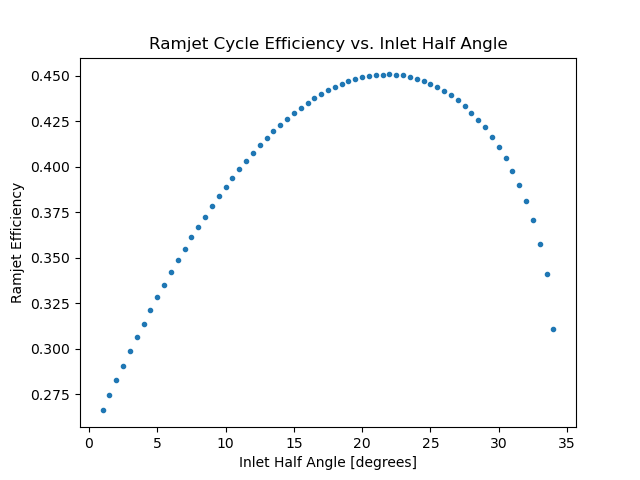
\includegraphics[]{../../images/problem_2/idealtheta.png}
    \caption{Ramjet cycle efficiency vs. inlet half-angle for Mach 3 cruise}
    \label{idealtheta}
\end{figure}

\end{enumerate}

\problempart{c} 

What is the efficiency of the ramjet if we get rid of the spike altogether?

\assumptions{}
Remove the inlet spike and corresponding oblique shock while retaining normal shock and all components downstream.

\solution{}
Repeat the solution procedure outlined in part (b), removing the oblique-shock relations and setting \(M_2 = M_1 = M_\infty\).
The ramjet cycle efficiency calculated with a normal shock inlet is 31.7\%. 
For the given flight condition there is only a single solution for cycle efficiency as the variable of inlet geometry has been removed.


\problempart{d} 

Write up a description of your observations of the ramjet with and without the spike.
Be sure to include relevant compressible-flow theories/jargon. 
Be sure to include a conversation of the effect of inlet freestream pressure ratio, inlet total pressure ratio, and combustor freestream temperature difference.

\discussion{}
The ramjet with the spike inlet shows a range of efficiencies that initially increases with inlet half angle and decreases beyond a turn angle of approximately 21 degrees.
For very small turn angles the oblique shock generated is very nearly a mach wave and does little to compress the flow which then goes through a stronger normal shock, similar to the case without the inlet spike.
At the upper end of the turn angle range, efficiences begin to fall off rapidly until the maximum turn angle is reached and the flow becomes separated from the inlet.
While the exact details of detached flow are not considered in this analysis, efficiences will tend towards a pure normal shock and dramatically less efficient performance.
The spike inlet geometry maintains a much higher inlet total pressure ratio than the normal shock case, which indicates that it is much more efficient.
For the ideal case, the efficiency is nearly 2x that of the normal shock case. 

The normal shock creates a generally larger inlet static pressure ratio, indicative of more compression.
Although this result is desirable, taken in conjunction with the total pressure recovery, the pure normal shock is less desirable.
The normal shock case has a smaller difference in freestream temperature across the combustion chamber compared to the inlet case.
In general, use of oblique shocks to compress and turn the flow is more efficient than a standing normal shock as entropy changes and total pressure loss are reduce for the oblique shock inlet.


\problempart{e} 

For the optimal spike half angle solved for in part (b), let's now explore the effect of cruise Mach number on efficiency. 
Plot efficiency versus cruise Mach number.

\solution{}
Using the methodology outlined in part (b), we vary Mach number with a fixed inlet half angle of 22 degrees.
The corresponding shock angle, \(\beta\), is be recalculated for each cruise Mach.
A range of Mach number \(2<M_\infty<6\) is analyzed, covering and exceeding the common ramjet operational range.
Figure \ref{eta_vs_mach} shows the relationship between ramjet cycle efficiency and cruise Mach number.
The maximum efficiency is 48.32\% at a cruise Mach number of \(M_\infty=3.4\).

\begin{figure}[h!]
    \centering
    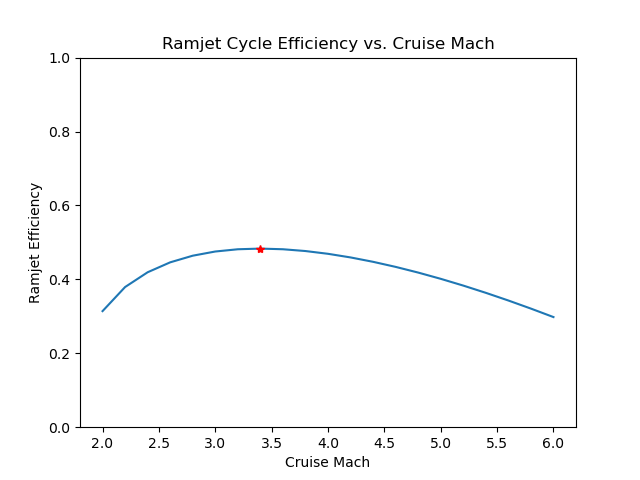
\includegraphics[]{../../images/problem_2/eta_vs_mach.png}
    \caption{Ramjet cycle efficiency vs. Cruise Mach}
    \label{eta_vs_mach}
\end{figure}

\problempart{f} 

Write up a description of your observations of the Mach-number effect on ramjets. 
Be sure to include the phenomena that limit the ramjet's performance at higher Mach numbers.
Be sure to include relevant compressible-flow theories/jargon. 
Be sure to include a conversation of the effect of inlet freestream pressure ratio, inlet total pressure ratio, and combustor freestream temperature difference.

\discussion{}
For a ramjet with a 21 degree inlet half angle the maximum efficiency is 48.32\% at a cruise Mach number of \(M_\infty=3.4\).
On either side of this ideal Mach number there is a reduced efficiency.
For smaller Mach numbers there is less compression generated by the shocks indicating that the ramjet inlet is less efficient at compression when operating below its design point. 
Larger Mach numbers cause the total pressure ratio \(\frac{p_{t,3}}{p_{t,1}}\) to become increasingly small as the shock strength grows larger.
The combustor static temperature difference increases with increasing cruise Mach, although the sensitivity of the ramjet's efficiency to this parameter is less obvious than the previous two.
As the temperature difference increases, the efficiency parameter goes down with it.
Ramjets are limited by the subsonic combustion requirement --- as \(M_\infty\) increases, the losses associated with reducing the flow to a subsonic velocity become large.
Scramjets are the solution to the getting around this efficiency issue as they are designed to operate with supersonic combustion.


\problempart{g} 

What do you expect to happen if we instead treat the spike as an axisymmetric cone?
Briefly justify your answer with words.

\discussion{}
If the inlet spike were treated as an axisymmetric cone instead of a 2-D wedge, the oblique shock would be weaker than the wedge case due to the 3-D relieving effects associated with the geometry.
Downstream static temperature and pressure would be smaller than the 2-D case, with a higher total pressure ratio across the shock. 
Although the weaker shock seems ideal from an efficiency standpoint, we may not be generating the ideal compression required and the downstream flow that passes through the standing normal shock would be at a higher Mach number and therefore experience a stronger shock than the 2-D case.
A solution would be to use a series of oblique shocks along a curved ramp instead of a linear cone to gradually induce compression and slow the flow more efficiently than a single oblique shock and a standing normal shock.


\end{document}